%    PACKAGES AND THEMES

\documentclass[aspectratio=169,xcolor=dvipsnames]{beamer}
\usetheme{Frankfurt}

\usepackage{hyperref}
\usepackage{verbatim}
\usepackage{graphicx}
\usepackage{array}
\usepackage{booktabs}
\usepackage{colortbl}
\usepackage{tikz}
\usepackage{amsmath}
\usetikzlibrary{arrows.meta,positioning,calc,backgrounds,shapes.geometric,shapes.multipart}
\setbeamersize{text margin left=3mm, text margin right=3mm}
\setbeamertemplate{headline}{}
\setbeamercovered{transparent=20}

\newcommand{\shellcmd}[1]{%
  \colorbox{black!10}{\parbox{0.93\linewidth}{\footnotesize\ttfamily #1}}%
}

%    TITLE PAGE

\title{Low-Overhead Dirty Access Tracking in GPU-UVM}
\author{Aditi Khandelia \and Arush Upadhyaya \and Kushagra Srivastava \and Sankalp Mittal \and Vidhi Jain}
\date{}
\institute
{
    \parbox{\textwidth}{\centering
    CS614 : Linux Kernel Programming \\
    Department of Computer Science and Engineering \\
    Indian Institute of Technology Kanpur}
}


%    PRESENTATION SLIDES

\begin{document}

\begin{frame}
    \titlepage
\end{frame}

\begin{frame}{Overview}
    \tableofcontents
\end{frame}

\section{Introduction}

\begin{frame}{Introduction}
\begin{itemize}
    \item NVIDIA's \textbf{Unified Virtual Memory (UVM)} subsystem underpins \texttt{cudaMallocManaged} and manages demand-paging between host and device via a hardware fault-driven path
    \item UVM exposes no interface for querying which pages a process has modified; any system requiring this must conservatively copy the \textbf{entire} GPU memory footprint
    \item We implement \textbf{per-process dirty page tracking} directly within the open-source NVIDIA UVM kernel module, augmenting the write-fault servicing path without additional hardware overhead
    \item Each recorded write carries a \textbf{nanosecond-resolution timestamp}, enabling precise ordering of writes across epochs and across CPU-GPU phases
    \item A \texttt{procfs}-based interface exposes start, stop, pause, resume, and atomic cutover snapshot operations to a privileged user with \textbf{page-level granularity}
\end{itemize}
\end{frame}

\section{Motivation}

% \begin{frame}{Motivation}{Why Dirty Tracking?}
% \begin{itemize}[<+->]
%     \item The Linux kernel tracks CPU dirty pages via soft-dirty bits in page-table entries, readable through \texttt{/proc/\textit{PID}/pagemap}; \textbf{no equivalent exists for GPU-managed memory}
%     \item Live process migration relies on identifying exactly which pages were written each round; without GPU dirty tracking, the entire GPU memory footprint must be copied conservatively on every iteration
%     \item Fault-tolerant ML training requires knowing which model-parameter pages were updated to enable \textbf{incremental checkpointing} and avoid full restart on failure
%     \item In heterogeneous CPU-GPU workloads with alternating compute phases, only GPU-written pages need to be synchronised back to the host; tracking eliminates unnecessary transfers
%     \item UVM already intercepts every GPU page fault for demand-paging, making the fault path a \textbf{natural and zero-hardware-cost} instrumentation point
% \end{itemize}
% \end{frame}

\begin{frame}{Motivation}{Limitations of Existing Approaches}
\begin{itemize}[<+->]
    \item \textbf{Full memory copy:} The only correct option today without tracking; conservatively transfers the entire allocation regardless of how little was actually written
    \item \textbf{Application-level bookkeeping:} Requires instrumenting every kernel call site to record writes; not transparent, breaks with third-party or compiled-only code
    \item \textbf{Sampling-based profilers (CUPTI, nvprof):} Impose high overhead, capture aggregate statistics rather than per-page write identity, and require profiling mode which is unavailable in production
    \item \textbf{Software checksumming:} Hashing memory regions to detect changes requires reading the entire allocation on every epoch boundary, producing overhead proportional to allocation size rather than write density
    \item \textbf{No epoch or timestamp support:} None of the above provide a mechanism to atomically snapshot the dirty set at an epoch boundary or order writes in time, both of which are required for correct iterative migration
\end{itemize}
\end{frame}



\section{Implementation}

\begin{frame}[c]{Implementation}{End-to-End Workflow}
\begin{center}
\resizebox{\textwidth}{!}{%
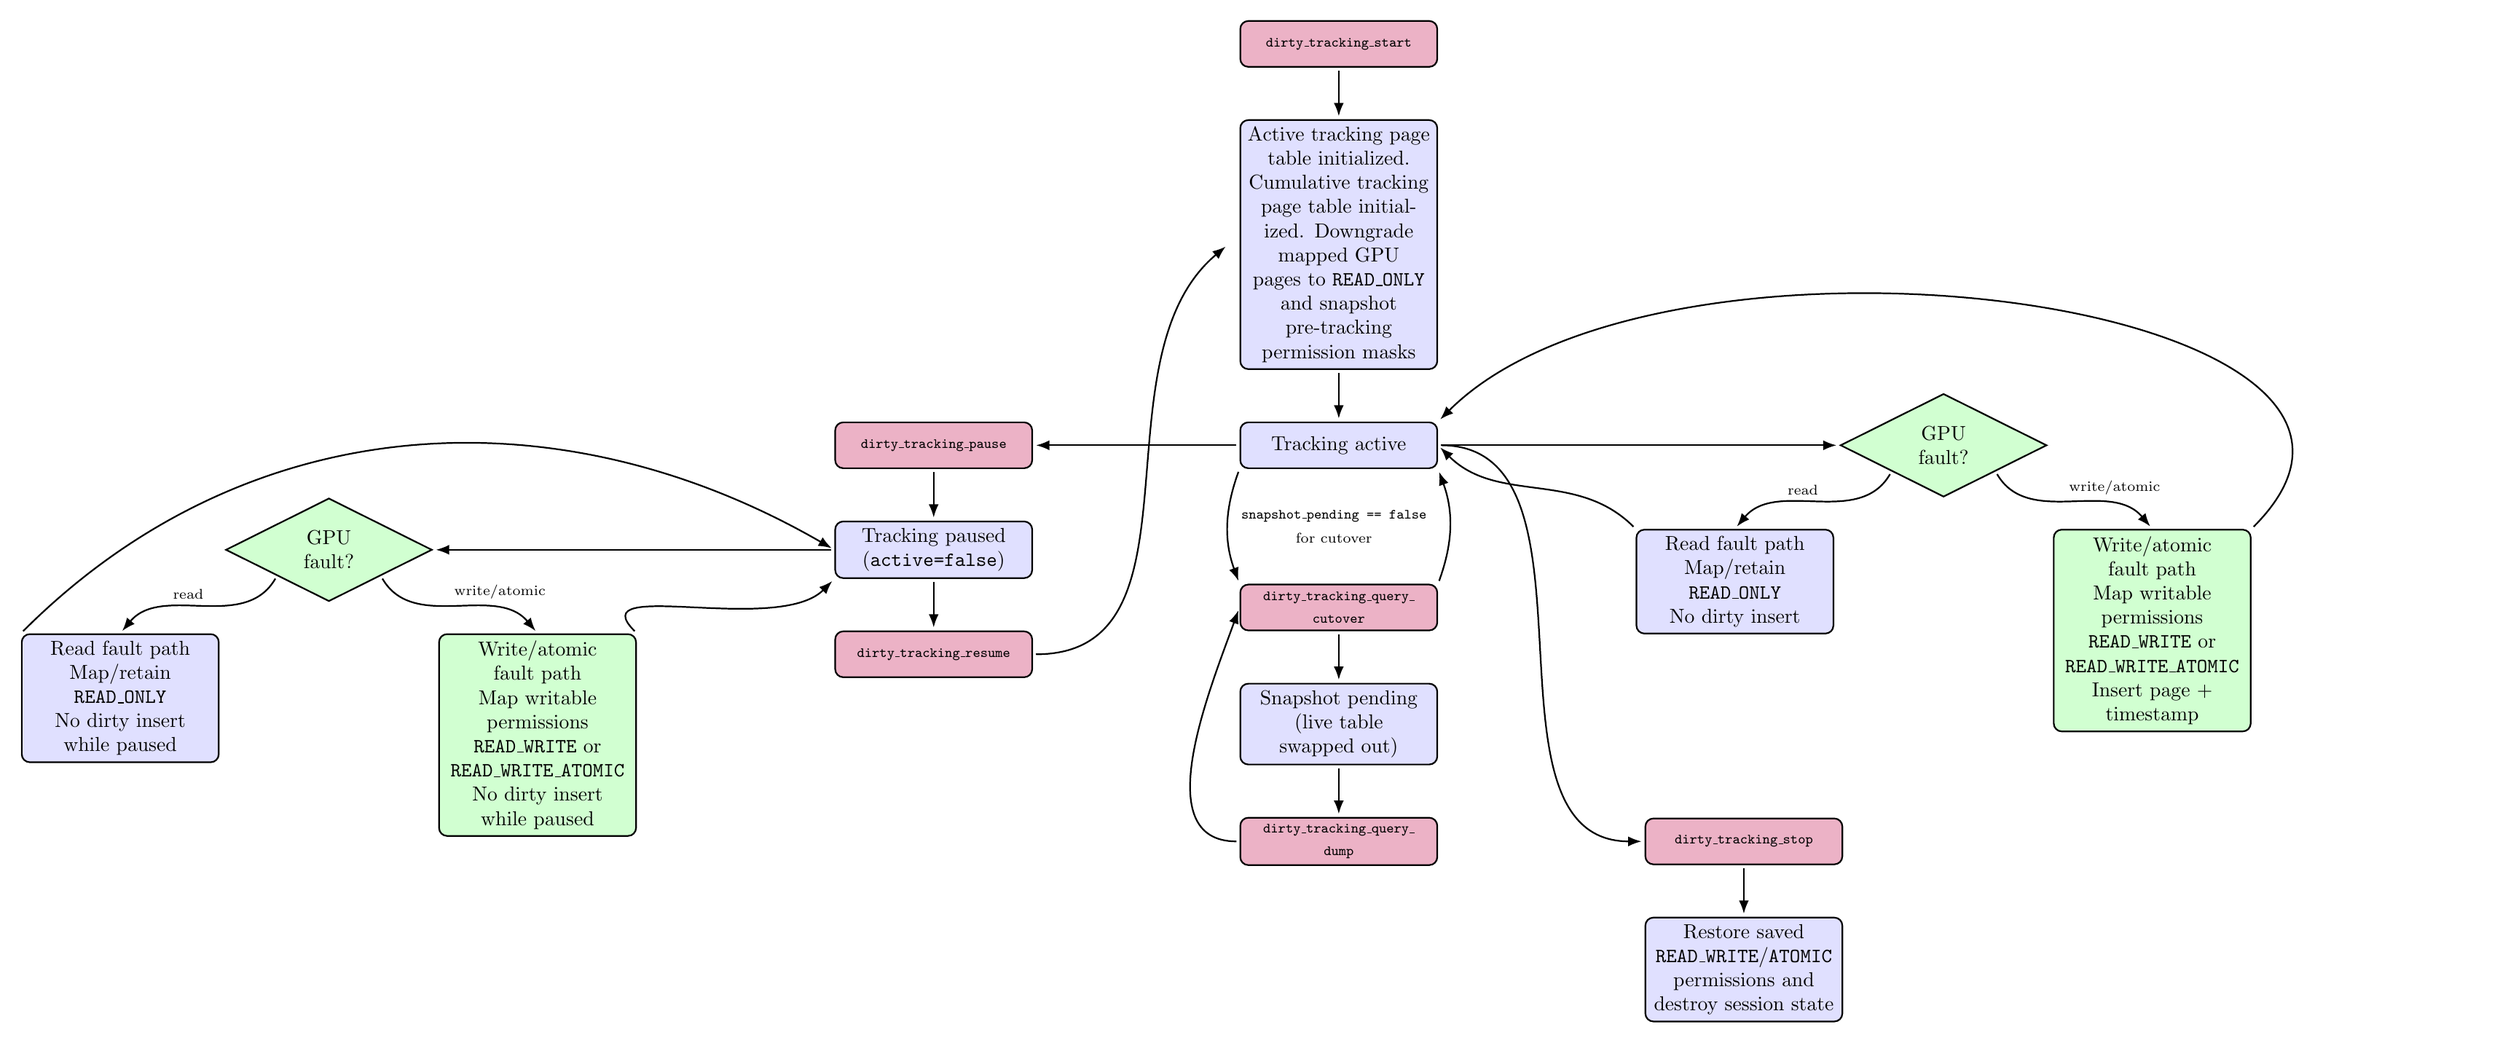
\begin{tikzpicture}[
    node distance=9mm and 10mm,
    box/.style={rectangle, rounded corners, draw=black, thick, align=center, text width=32mm, minimum height=8mm, fill=blue!12},
    readbox/.style={box, fill=blue!12},
    writebox/.style={box, fill=green!18},
    procfs/.style={box, fill=purple!30},
    decision/.style={shape=diamond, draw=black, thick, fill=green!18, aspect=2.0, align=center, inner sep=1.3pt, text width=20mm},
    flow/.style={-Latex, thick, shorten >=1.5pt, shorten <=1.5pt}
]

\node[procfs] (start) {{\scriptsize\texttt{dirty\_tracking\_start}}};
\node[box, below=of start] (downgrade) {Active tracking page table initialized. Cumulative tracking page table initialized. Downgrade mapped GPU pages to \texttt{READ\_ONLY}\\and snapshot pre-tracking permission masks};
\node[box, below=of downgrade] (active) {Tracking active};

\node[procfs, left=36mm of active] (pausecmd) {{\scriptsize\texttt{dirty\_tracking\_pause}}};
\node[box, below=of pausecmd] (paused) {Tracking paused\\(\texttt{active=false})};
\node[procfs, below=of paused] (resume) {{\scriptsize\texttt{dirty\_tracking\_resume}}};

\node[procfs, below=20mm of active] (cutover) {{\scriptsize\texttt{dirty\_tracking\_query\_}}\\[-1pt]{\scriptsize\texttt{cutover}}};
\node[box, below=of cutover] (snapshot) {Snapshot pending\\(live table swapped out)};
\node[procfs, below=of snapshot] (dump) {{\scriptsize\texttt{dirty\_tracking\_query\_}}\\[-1pt]{\scriptsize\texttt{dump}}};

\node[decision, right=70mm of active] (access) {GPU\\fault?};
\node[readbox, below left=10mm and 10mm of access] (readpath) {Read fault path\\Map/retain \texttt{READ\_ONLY}\\No dirty insert};
\node[writebox, below right=10mm and 10mm of access] (writepath) {Write/atomic fault path\\Map writable permissions \texttt{READ\_WRITE} or \texttt{READ\_WRITE\_ATOMIC}\\Insert page + timestamp};

\node[decision, left=70mm of paused] (pausedaccess) {GPU\\fault?};
\node[readbox, below left=10mm and 10mm of pausedaccess] (pausedreadpath) {Read fault path\\Map/retain \texttt{READ\_ONLY}\\No dirty insert while paused};
\node[writebox, below right=10mm and 10mm of pausedaccess] (pausedwritepath) {Write/atomic fault path\\Map writable permissions\\\texttt{READ\_WRITE} or \texttt{READ\_WRITE\_ATOMIC}\\No dirty insert while paused};

\node[procfs, right=36mm of dump] (stop) {{\scriptsize\texttt{dirty\_tracking\_stop}}};
\node[box, below=of stop] (restore) {Restore saved \texttt{READ\_WRITE}/\texttt{ATOMIC}\\permissions and destroy session state};

\draw[flow] (start) -- (downgrade);
\draw[flow] (downgrade) -- (active);

\draw[flow] (active.west) -- (pausecmd.east);
\draw[flow] (pausecmd) -- (paused);
\draw[flow] (paused) -- (resume);
\draw[flow] (resume.east) to[out=0,in=220] ([xshift=-2mm]downgrade.west);

\draw[flow] (active.south west) to[out=-110,in=110]
    node[pos=0.5, right=1mm, align=center] {\scriptsize \texttt{snapshot\_pending == false}\\\scriptsize{for cutover}}
    (cutover.north west);
\draw[flow] (cutover.north east) to[out=70,in=-70] (active.south east);
\draw[flow] (cutover) -- (snapshot);
\draw[flow] (snapshot) -- (dump);
\draw[flow] (dump.west) to[out=180,in=-110] (cutover.west);

\draw[flow] (active.east) -- (access.west);
\draw[flow] (access.south west) to[out=240,in=50] node[above left, pos=0.45] {\scriptsize read} (readpath.north);
\draw[flow] (access.south east) to[out=300,in=130] node[above right, pos=0.45] {\scriptsize write/atomic} (writepath.north);
\draw[flow] (readpath.north west) to[out=135,in=-45] (active.east);
\draw[flow] (writepath.north east) to[out=45,in=45] (active.north east);

\draw[flow] (paused.west) -- (pausedaccess.east);
\draw[flow] (pausedaccess.south west) to[out=240,in=50] node[above left, pos=0.45] {\scriptsize read} (pausedreadpath.north);
\draw[flow] (pausedaccess.south east) to[out=300,in=130] node[above right, pos=0.45] {\scriptsize write/atomic} (pausedwritepath.north);
\draw[flow] (pausedreadpath.north west) to[out=45,in=150] (paused.west);
\draw[flow] (pausedwritepath.north east) to[out=135,in=-135] (paused.south west);

\draw[flow] (active.east) to[out=0,in=180] (stop.west);
\draw[flow] (stop) -- (restore);

\end{tikzpicture}
}
\end{center}
\end{frame}

\begin{frame}[c]{Implementation}{State Transition Diagram}
\begin{center}
\resizebox{0.72\textwidth}{!}{%
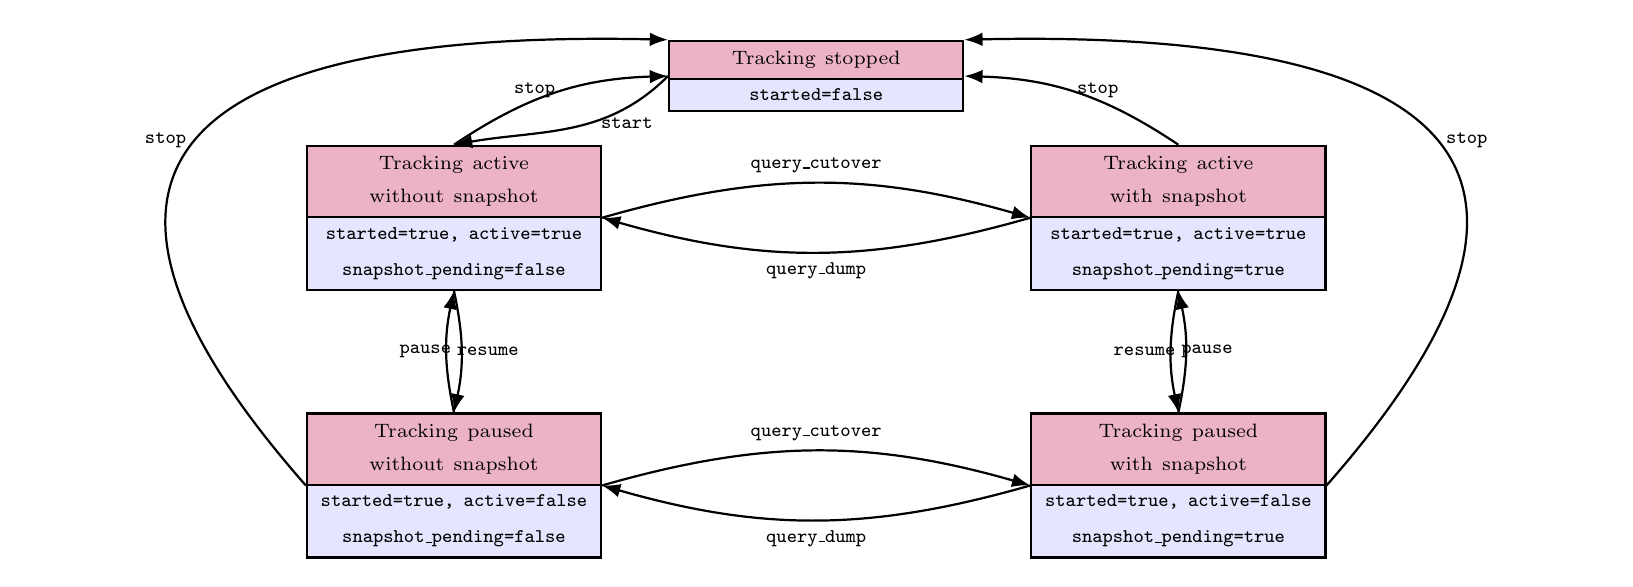
\begin{tikzpicture}[
    st/.style={rectangle split, rectangle split parts=2,
               rectangle split part fill={purple!30, blue!10},
               draw=black, thick, align=center, text width=35mm},
    tr/.style={-Latex, thick}
]
\node[st] (stopped) at (0mm,22mm)
    {{\scriptsize Tracking stopped}
     \nodepart{two}{\scriptsize \texttt{started=false}}};
\node[st] (active_no) at (-46mm,4mm)
    {{\scriptsize Tracking active without snapshot}
     \nodepart{two}{\scriptsize \texttt{started=true, active=true}\\[1pt]\texttt{snapshot\_pending=false}}};
\node[st] (active_yes) at (46mm,4mm)
    {{\scriptsize Tracking active with snapshot}
     \nodepart{two}{\scriptsize \texttt{started=true, active=true}\\[1pt]\texttt{snapshot\_pending=true}}};
\node[st] (paused_no) at (-46mm,-30mm)
    {{\scriptsize Tracking paused without snapshot}
     \nodepart{two}{\scriptsize \texttt{started=true, active=false}\\[1pt]\texttt{snapshot\_pending=false}}};
\node[st] (paused_yes) at (46mm,-30mm)
    {{\scriptsize Tracking paused with snapshot}
     \nodepart{two}{\scriptsize \texttt{started=true, active=false}\\[1pt]\texttt{snapshot\_pending=true}}};

\draw[tr] (stopped.west) to[out=225,in=10] node[right, pos=0.40] {\scriptsize \texttt{start}} (active_no.north);

\draw[tr] (active_no.east) to[bend left=16] node[above] {\scriptsize \texttt{query\_cutover}} (active_yes.west);
\draw[tr] (active_yes.west) to[bend left=16] node[below] {\scriptsize \texttt{query\_dump}} (active_no.east);
\draw[tr] (paused_no.east) to[bend left=16] node[above] {\scriptsize \texttt{query\_cutover}} (paused_yes.west);
\draw[tr] (paused_yes.west) to[bend left=16] node[below] {\scriptsize \texttt{query\_dump}} (paused_no.east);

\draw[tr] (active_no.south) to[bend left=12] node[left] {\scriptsize \texttt{pause}} (paused_no.north);
\draw[tr] (paused_no.north) to[bend left=12] node[right] {\scriptsize \texttt{resume}} (active_no.south);
\draw[tr] (active_yes.south) to[bend right=12] node[right] {\scriptsize \texttt{pause}} (paused_yes.north);
\draw[tr] (paused_yes.north) to[bend right=12] node[left] {\scriptsize \texttt{resume}} (active_yes.south);

\draw[tr] (active_no.north) to[bend left=16] node[left, pos=0.55] {\scriptsize \texttt{stop}} (stopped.west);
\draw[tr] (active_yes.north) to[bend right=16] node[right, pos=0.55] {\scriptsize \texttt{stop}} (stopped.east);
\draw[tr] (paused_no.west) .. controls (-100mm,10mm) and (-82mm,28mm) ..
    node[left, pos=0.5] {\scriptsize \texttt{stop}} (stopped.north west);
\draw[tr] (paused_yes.east) .. controls (100mm,10mm) and (82mm,28mm) ..
    node[right, pos=0.5] {\scriptsize \texttt{stop}} (stopped.north east);
\end{tikzpicture}
}
\end{center}
\vspace{2mm}
{\small All lifecycle operations are serialised by \texttt{uvm\_dirty\_lifecycle\_lock}. Transitions that violate owner checks, state preconditions, or snapshot guards are rejected by the procfs handlers.}
\end{frame}

\begin{frame}[c]{Implementation}{Permission Lifecycle (1/2)}
\begin{center}
\renewcommand{\arraystretch}{1.3}
\footnotesize
\begin{tabular}{p{22mm} p{58mm} p{52mm}}
\toprule
\textbf{Phase} & \textbf{GPU Page Permission} & \textbf{Dirty Recording} \\
\midrule
\textbf{start / resume} &
    Save \texttt{pte\_bits[WRITE/ATOMIC]} into \texttt{dirty\_downgraded\_pages}; revoke write perms $\to$ \texttt{READ\_ONLY} &
    Tables initialised; \texttt{active=true} \\
\textbf{Read fault} &
    Forced \texttt{READ\_ONLY} (\texttt{uvm\_va\_block.c}) &
    Not inserted \\
\textbf{Write fault} &
    Restored to \texttt{READ\_WRITE} / \texttt{ATOMIC} (\texttt{uvm\_gpu\_replayable\_faults.c}) &
    \texttt{page\_num + ktime\_get\_ns()} inserted (first-write-wins) \\
\textbf{Prefetch} &
    GPU-migrated pages mapped \texttt{READ\_ONLY} (\texttt{uvm\_migrate.c}) &
    Not inserted; write fault records on first write \\
\textbf{pause} &
    Write faults still grant \texttt{READ\_WRITE}/\texttt{ATOMIC} for forward progress &
    Not inserted (\texttt{active=false}); query barrier drains fault buffer first \\
\bottomrule
\end{tabular}
\end{center}
\end{frame}

\begin{frame}[c]{Implementation}{Permission Lifecycle (2/2)}
\begin{center}
\renewcommand{\arraystretch}{1.3}
\footnotesize
\begin{tabular}{p{22mm} p{58mm} p{52mm}}
\toprule
\textbf{Phase} & \textbf{GPU Page Permission} & \textbf{Dirty Recording} \\
\midrule
\textbf{resume} &
    Re-runs downgrade sequence; \texttt{READ\_ONLY} re-armed without reinitialising tables &
    Recording resumes; \texttt{active=true} \\
\textbf{cutover} &
    No change &
    Live $\to$ snapshot under query barrier; fresh live table installed; \texttt{snapshot\_pending=true} \\
\textbf{dump} &
    No change &
    Delta: emit snapshot. Cumulative: merge into cumulative (first-write-wins), emit union \\
\textbf{stop} &
    Walk VA blocks; restore \texttt{dirty\_downgraded\_pages} masks; exact pre-tracking perms recovered &
    All tables destroyed; state reset \\
\bottomrule
\end{tabular}
\end{center}
\end{frame}

\begin{frame}{Implementation}{Procfs Interface: Lifecycle Controls}
\begin{block}{\texttt{dirty\_tracking\_start}}
    \footnotesize
    \shellcmd{echo "<PID> delta|cumulative" > /proc/driver/nvidia-uvm/dirty\_tracking\_start}\\[2pt]
    Initialises live table; downgrades all GPU PTEs to \texttt{READ\_ONLY} and saves per-page PTE masks; sets \texttt{active=true}. Mode selects delta (per-epoch diff) or cumulative (session union).
\end{block}
\vspace{2pt}
\pause
\begin{block}{\texttt{dirty\_tracking\_pause}}
    \footnotesize
    \shellcmd{echo "<PID>" > /proc/driver/nvidia-uvm/dirty\_tracking\_pause}\\[2pt]
    Acquires query barrier (locks ISRs, drains fault buffer); sets \texttt{active=false}. Faults still serviced for forward progress but no dirty inserts emitted.
\end{block}
\vspace{2pt}
\pause
\begin{block}{\texttt{dirty\_tracking\_resume}}
    \footnotesize
    \shellcmd{echo "<PID>" > /proc/driver/nvidia-uvm/dirty\_tracking\_resume}\\[2pt]
    Re-runs downgrade sequence (revoke PTEs, set \texttt{active=true}) without reinitialising tables. Entries accumulated before pause are preserved.
\end{block}
\end{frame}

\begin{frame}{Implementation}{Procfs Interface: Query Controls}
\begin{block}{\texttt{dirty\_tracking\_stop}}
    \footnotesize
    \shellcmd{echo "<PID>" > /proc/driver/nvidia-uvm/dirty\_tracking\_stop}\\[2pt]
    Restores exact pre-tracking permissions from \texttt{dirty\_downgraded\_pages} masks; destroys live, snapshot, and cumulative tables; flushes stats to \texttt{/tmp/uvm\_dirty\_ds\_stats.txt}.
\end{block}
\vspace{2pt}
\pause
\begin{block}{\texttt{dirty\_tracking\_query\_cutover}}
    \footnotesize
    \shellcmd{echo "<PID>" > /proc/driver/nvidia-uvm/dirty\_tracking\_query\_cutover}\\[2pt]
    Acquires query barrier; atomically swaps live $\to$ snapshot and installs a fresh live table; increments epoch counter; sets \texttt{snapshot\_pending=true}.
\end{block}
\vspace{2pt}
\pause
\begin{block}{\texttt{dirty\_tracking\_query\_dump}}
    \footnotesize
    \shellcmd{cat /proc/driver/nvidia-uvm/dirty\_tracking\_query\_dump}\\[2pt]
    Emits frozen snapshot as \texttt{0x<addr> <timestamp\_ns>} lines. Delta: snapshot only. Cumulative: merge into session-union (first-write-wins) then emit union. Overflow-safe: snapshot retained and replayed on \texttt{seq\_file} overflow.
\end{block}
\end{frame}

\begin{frame}{Implementation}{Procfs Interface: Instrumentation and Backend}
\begin{block}{\texttt{dirty\_ds\_stats\_toggle}}
    \footnotesize
    \shellcmd{echo "enable|disable" > /proc/driver/nvidia-uvm/dirty\_ds\_stats\_toggle}\\[2pt]
    \texttt{enable}: resets all atomic counters and starts accumulation. \texttt{disable}: halts accumulation. Covers insert, lookup, for-each, init, destroy, and callback timing.
\end{block}
\vspace{2pt}
\pause
\begin{block}{\texttt{dirty\_ds\_stats}}
    \footnotesize
    \shellcmd{cat /proc/driver/nvidia-uvm/dirty\_ds\_stats}\\[2pt]
    Prints per-operation call count, average latency (ns), and average \texttt{rwsem} wait time. Also reports average latency for invalidate, activate-now, and barrier-end callbacks.
\end{block}
\vspace{2pt}
\pause
\begin{block}{\texttt{dirty\_tracking\_hint}}
    \footnotesize
    \shellcmd{echo "WRITE\_SEQ|WRITE\_RAND" > /proc/driver/nvidia-uvm/dirty\_tracking\_hint}\\[2pt]
    Switches backend before a session. \texttt{WRITE\_SEQ} $\to$ sorted vector (sequential workloads); \texttt{WRITE\_RAND} $\to$ nested bitmap (random workloads). Rejected if any table is initialised.
\end{block}
\end{frame}

\section{Design Choices}

\begin{frame}[c]{Design Choices}{Determinism in \texttt{start} and \texttt{resume}}
\begin{columns}[c]

\column{0.48\textwidth}
\centering
{\footnotesize\textbf{\texttt{dirty\_tracking\_start}}}\\[2pt]
\resizebox{!}{0.7\textheight}{%
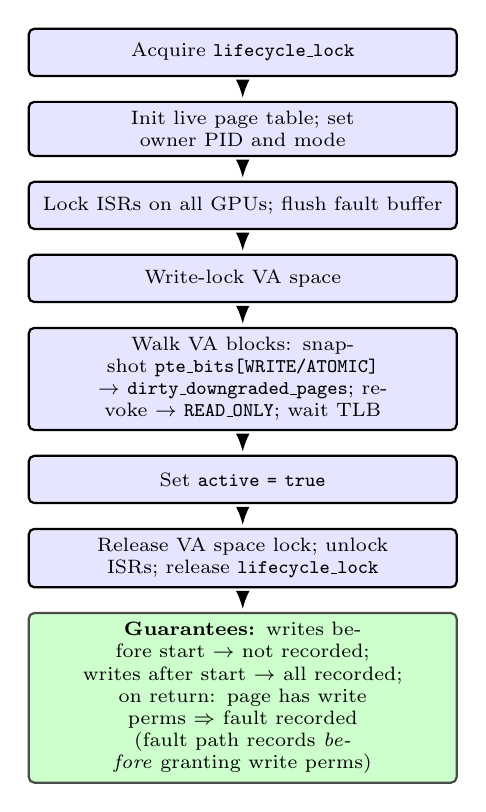
\begin{tikzpicture}[
    node distance=3mm,
    box/.style={rectangle, rounded corners=2pt, draw=black, thick, fill=blue!10,
                align=center, text width=52mm, minimum height=6mm, font=\scriptsize},
    gbox/.style={rectangle, rounded corners=2pt, draw=black!70, thick, fill=green!20,
                 align=center, text width=52mm, minimum height=7mm, font=\scriptsize},
    flow/.style={-Latex, thick, shorten >=1pt, shorten <=1pt}
]
\node[box] (s1) {Acquire \texttt{lifecycle\_lock}};
\node[box, below=of s1] (s2) {Init live page table; set owner PID and mode};
\node[box, below=of s2] (s3) {Lock ISRs on all GPUs; flush fault buffer};
\node[box, below=of s3] (s4) {Write-lock VA space};
\node[box, below=of s4] (s5) {Walk VA blocks: snapshot \texttt{pte\_bits[WRITE/ATOMIC]}\\$\to$ \texttt{dirty\_downgraded\_pages}; revoke $\to$ \texttt{READ\_ONLY}; wait TLB};
\node[box, below=of s5] (s6) {Set \texttt{active = true}};
\node[box, below=of s6] (s7) {Release VA space lock; unlock ISRs; release \texttt{lifecycle\_lock}};
\node[gbox, below=3mm of s7] (sg) {\textbf{Guarantees:} writes before start $\to$ not recorded;\\writes after start $\to$ all recorded;\\on return: page has write perms $\Rightarrow$ fault recorded\\(fault path records \emph{before} granting write perms)};
\draw[flow] (s1)--(s2); \draw[flow] (s2)--(s3); \draw[flow] (s3)--(s4);
\draw[flow] (s4)--(s5); \draw[flow] (s5)--(s6); \draw[flow] (s6)--(s7); \draw[flow] (s7)--(sg);
\end{tikzpicture}}

\pause
\column{0.48\textwidth}
\centering
{\footnotesize\textbf{\texttt{dirty\_tracking\_resume}}}\\[2pt]
\resizebox{!}{0.7\textheight}{%
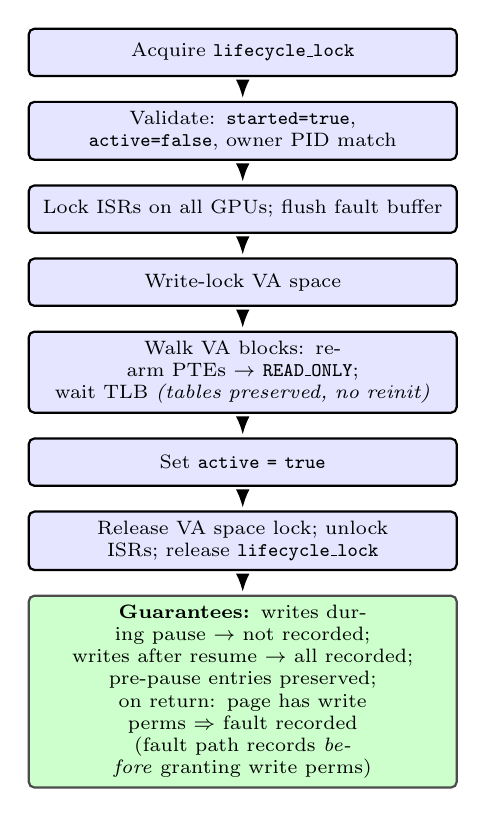
\begin{tikzpicture}[
    node distance=3mm,
    box/.style={rectangle, rounded corners=2pt, draw=black, thick, fill=blue!10,
                align=center, text width=52mm, minimum height=6mm, font=\scriptsize},
    gbox/.style={rectangle, rounded corners=2pt, draw=black!70, thick, fill=green!20,
                 align=center, text width=52mm, minimum height=7mm, font=\scriptsize},
    flow/.style={-Latex, thick, shorten >=1pt, shorten <=1pt}
]
\node[box] (r1) {Acquire \texttt{lifecycle\_lock}};
\node[box, below=of r1] (r2) {Validate: \texttt{started=true}, \texttt{active=false}, owner PID match};
\node[box, below=of r2] (r3) {Lock ISRs on all GPUs; flush fault buffer};
\node[box, below=of r3] (r4) {Write-lock VA space};
\node[box, below=of r4] (r5) {Walk VA blocks: re-arm PTEs $\to$ \texttt{READ\_ONLY};\\wait TLB \emph{(tables preserved, no reinit)}};
\node[box, below=of r5] (r6) {Set \texttt{active = true}};
\node[box, below=of r6] (r7) {Release VA space lock; unlock ISRs; release \texttt{lifecycle\_lock}};
\node[gbox, below=3mm of r7] (rg) {\textbf{Guarantees:} writes during pause $\to$ not recorded;\\writes after resume $\to$ all recorded; pre-pause entries preserved;\\on return: page has write perms $\Rightarrow$ fault recorded\\(fault path records \emph{before} granting write perms)};
\draw[flow] (r1)--(r2); \draw[flow] (r2)--(r3); \draw[flow] (r3)--(r4);
\draw[flow] (r4)--(r5); \draw[flow] (r5)--(r6); \draw[flow] (r6)--(r7); \draw[flow] (r7)--(rg);
\end{tikzpicture}}

\end{columns}
\end{frame}

\begin{frame}[c]{Design Choices}{Determinism in \texttt{pause} and \texttt{stop}}
\begin{columns}[c]

\column{0.48\textwidth}
\centering
{\footnotesize\textbf{\texttt{dirty\_tracking\_pause}}}\\[2pt]
\resizebox{!}{0.7\textheight}{%
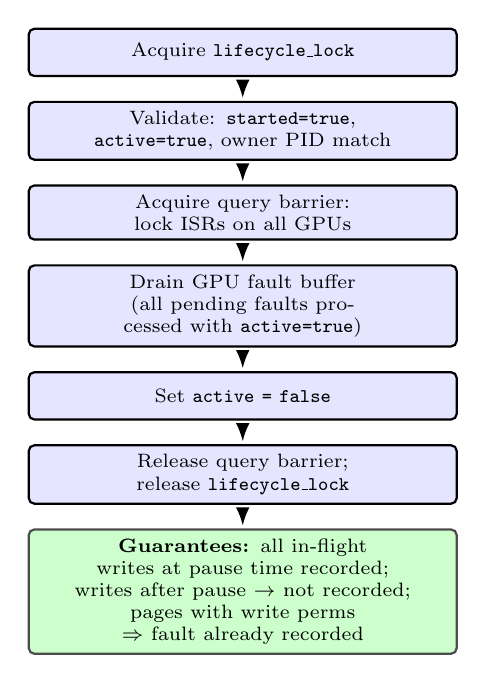
\begin{tikzpicture}[
    node distance=3mm,
    box/.style={rectangle, rounded corners=2pt, draw=black, thick, fill=blue!10,
                align=center, text width=52mm, minimum height=6mm, font=\scriptsize},
    gbox/.style={rectangle, rounded corners=2pt, draw=black!70, thick, fill=green!20,
                 align=center, text width=52mm, minimum height=7mm, font=\scriptsize},
    flow/.style={-Latex, thick, shorten >=1pt, shorten <=1pt}
]
\node[box] (p1) {Acquire \texttt{lifecycle\_lock}};
\node[box, below=of p1] (p2) {Validate: \texttt{started=true}, \texttt{active=true}, owner PID match};
\node[box, below=of p2] (p3) {Acquire query barrier: lock ISRs on all GPUs};
\node[box, below=of p3] (p4) {Drain GPU fault buffer\\(all pending faults processed with \texttt{active=true})};
\node[box, below=of p4] (p5) {Set \texttt{active = false}};
\node[box, below=of p5] (p6) {Release query barrier; release \texttt{lifecycle\_lock}};
\node[gbox, below=3mm of p6] (pg) {\textbf{Guarantees:} all in-flight writes at pause time recorded;\\writes after pause $\to$ not recorded;\\pages with write perms $\Rightarrow$ fault already recorded};
\draw[flow] (p1)--(p2); \draw[flow] (p2)--(p3); \draw[flow] (p3)--(p4);
\draw[flow] (p4)--(p5); \draw[flow] (p5)--(p6); \draw[flow] (p6)--(pg);
\end{tikzpicture}}

\pause
\column{0.48\textwidth}
\centering
{\footnotesize\textbf{\texttt{dirty\_tracking\_stop}}}\\[2pt]
\resizebox{!}{0.7\textheight}{%
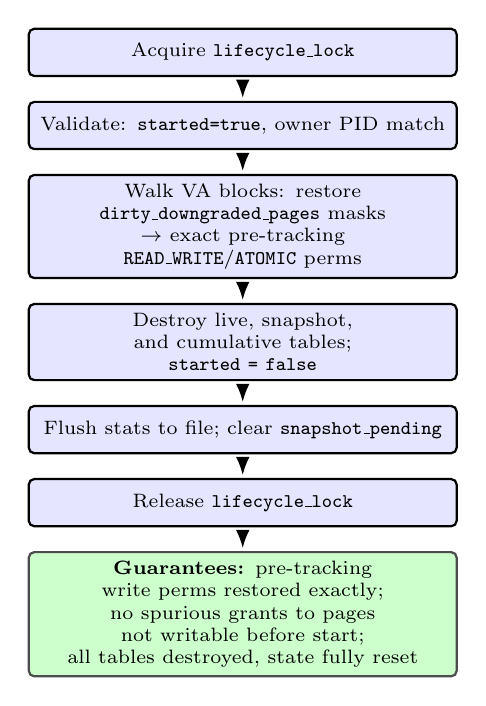
\begin{tikzpicture}[
    node distance=3mm,
    box/.style={rectangle, rounded corners=2pt, draw=black, thick, fill=blue!10,
                align=center, text width=52mm, minimum height=6mm, font=\scriptsize},
    gbox/.style={rectangle, rounded corners=2pt, draw=black!70, thick, fill=green!20,
                 align=center, text width=52mm, minimum height=7mm, font=\scriptsize},
    flow/.style={-Latex, thick, shorten >=1pt, shorten <=1pt}
]
\node[box] (t1) {Acquire \texttt{lifecycle\_lock}};
\node[box, below=of t1] (t2) {Validate: \texttt{started=true}, owner PID match};
\node[box, below=of t2] (t3) {Walk VA blocks: restore \texttt{dirty\_downgraded\_pages} masks\\$\to$ exact pre-tracking \texttt{READ\_WRITE}/\texttt{ATOMIC} perms};
\node[box, below=of t3] (t4) {Destroy live, snapshot, and cumulative tables;\\\texttt{started = false}};
\node[box, below=of t4] (t5) {Flush stats to file; clear \texttt{snapshot\_pending}};
\node[box, below=of t5] (t6) {Release \texttt{lifecycle\_lock}};
\node[gbox, below=3mm of t6] (tg) {\textbf{Guarantees:} pre-tracking write perms restored exactly;\\no spurious grants to pages not writable before start;\\all tables destroyed, state fully reset};
\draw[flow] (t1)--(t2); \draw[flow] (t2)--(t3); \draw[flow] (t3)--(t4);
\draw[flow] (t4)--(t5); \draw[flow] (t5)--(t6); \draw[flow] (t6)--(tg);
\end{tikzpicture}}

\end{columns}
\end{frame}

\begin{frame}[c]{Design Choices}{Atomicity in \texttt{query\_cutover} and \texttt{query\_dump}}
\begin{columns}[c]

\column{0.48\textwidth}
\centering
{\footnotesize\textbf{\texttt{dirty\_tracking\_query\_cutover}}}\\[2pt]
\resizebox{!}{0.7\textheight}{%
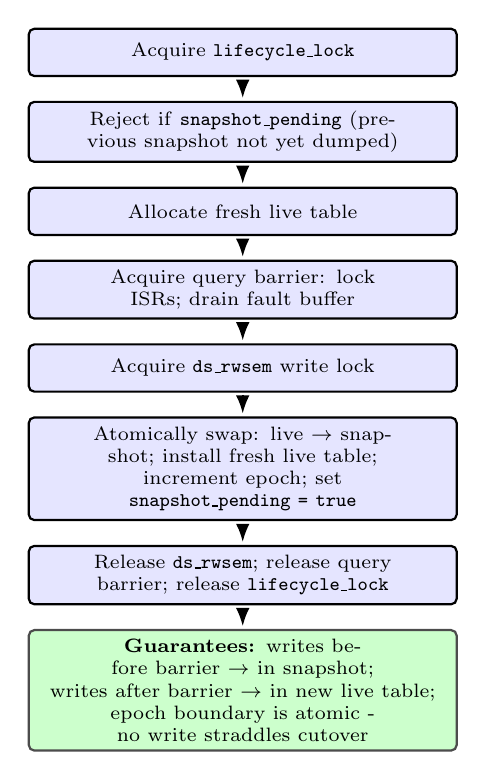
\begin{tikzpicture}[
    node distance=3mm,
    box/.style={rectangle, rounded corners=2pt, draw=black, thick, fill=blue!10,
                align=center, text width=52mm, minimum height=6mm, font=\scriptsize},
    gbox/.style={rectangle, rounded corners=2pt, draw=black!70, thick, fill=green!20,
                 align=center, text width=52mm, minimum height=7mm, font=\scriptsize},
    flow/.style={-Latex, thick, shorten >=1pt, shorten <=1pt}
]
\node[box] (c1) {Acquire \texttt{lifecycle\_lock}};
\node[box, below=of c1] (c2) {Reject if \texttt{snapshot\_pending} (previous snapshot not yet dumped)};
\node[box, below=of c2] (c3) {Allocate fresh live table};
\node[box, below=of c3] (c4) {Acquire query barrier: lock ISRs; drain fault buffer};
\node[box, below=of c4] (c5) {Acquire \texttt{ds\_rwsem} write lock};
\node[box, below=of c5] (c6) {Atomically swap: live $\to$ snapshot; install fresh live table;\\increment epoch; set \texttt{snapshot\_pending = true}};
\node[box, below=of c6] (c7) {Release \texttt{ds\_rwsem}; release query barrier; release \texttt{lifecycle\_lock}};
\node[gbox, below=3mm of c7] (cg) {\textbf{Guarantees:} writes before barrier $\to$ in snapshot;\\writes after barrier $\to$ in new live table;\\epoch boundary is atomic - no write straddles cutover};
\draw[flow] (c1)--(c2); \draw[flow] (c2)--(c3); \draw[flow] (c3)--(c4);
\draw[flow] (c4)--(c5); \draw[flow] (c5)--(c6); \draw[flow] (c6)--(c7); \draw[flow] (c7)--(cg);
\end{tikzpicture}}

\pause
\column{0.48\textwidth}
\centering
{\footnotesize\textbf{\texttt{dirty\_tracking\_query\_dump}}}\\[2pt]
\resizebox{!}{0.7\textheight}{%
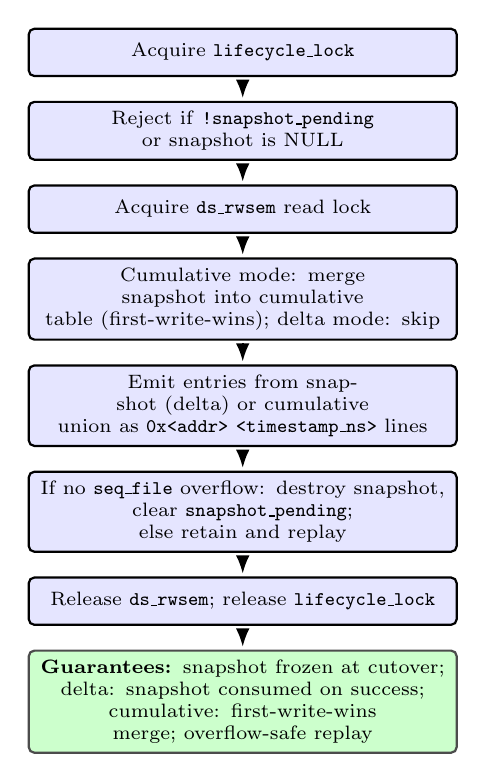
\begin{tikzpicture}[
    node distance=3mm,
    box/.style={rectangle, rounded corners=2pt, draw=black, thick, fill=blue!10,
                align=center, text width=52mm, minimum height=6mm, font=\scriptsize},
    gbox/.style={rectangle, rounded corners=2pt, draw=black!70, thick, fill=green!20,
                 align=center, text width=52mm, minimum height=7mm, font=\scriptsize},
    flow/.style={-Latex, thick, shorten >=1pt, shorten <=1pt}
]
\node[box] (d1) {Acquire \texttt{lifecycle\_lock}};
\node[box, below=of d1] (d2) {Reject if \texttt{!snapshot\_pending} or snapshot is NULL};
\node[box, below=of d2] (d3) {Acquire \texttt{ds\_rwsem} read lock};
\node[box, below=of d3] (d4) {Cumulative mode: merge snapshot into cumulative\\table (first-write-wins); delta mode: skip};
\node[box, below=of d4] (d5) {Emit entries from snapshot (delta) or cumulative\\union as \texttt{0x<addr> <timestamp\_ns>} lines};
\node[box, below=of d5] (d6) {If no \texttt{seq\_file} overflow: destroy snapshot,\\clear \texttt{snapshot\_pending}; else retain and replay};
\node[box, below=of d6] (d7) {Release \texttt{ds\_rwsem}; release \texttt{lifecycle\_lock}};
\node[gbox, below=3mm of d7] (dg) {\textbf{Guarantees:} snapshot frozen at cutover;\\delta: snapshot consumed on success;\\cumulative: first-write-wins merge; overflow-safe replay};
\draw[flow] (d1)--(d2); \draw[flow] (d2)--(d3); \draw[flow] (d3)--(d4);
\draw[flow] (d4)--(d5); \draw[flow] (d5)--(d6); \draw[flow] (d6)--(d7); \draw[flow] (d7)--(dg);
\end{tikzpicture}}

\end{columns}
\end{frame}

\begin{frame}{Design Choices}{Handling Prefetch (\texttt{cudaMemPrefetchAsync})}
\begin{itemize}[<+->]
    \item \texttt{cudaMemPrefetchAsync} migrates pages to the GPU without a fault - it calls into the migration path directly and maps pages \texttt{READ\_WRITE\_ATOMIC}, bypassing \texttt{compute\_new\_permission} and making any subsequent write \textbf{invisible} to the tracker
    \item Fix: in \texttt{uvm\_migrate.c}, when dirty tracking is started and the destination is a GPU, the migration path forces \texttt{prot = UVM\_PROT\_READ\_ONLY} instead of \texttt{READ\_WRITE\_ATOMIC} for all prefetched pages
    \item The first GPU write to a prefetched page then generates a write fault, which is intercepted by the fault handler - the page and its timestamp are recorded, and write permissions are restored exactly as they would be for a demand-paged write
    \item This preserves the core invariant: \textbf{a page can only acquire write permissions by going through the recorded fault path}, regardless of whether it arrived via demand-paging or prefetch
\end{itemize}
\end{frame}

\begin{frame}{Design Choices}{Query Modes}
\end{frame}

\begin{frame}{Design Choices}{Concurrency Design}
\end{frame}

\section{Data Structures and Associated Operations}
\begin{frame}{Data Structures and Associated Operations}{Overview}
\end{frame}

\section{Testing and Analysis}
\begin{frame}{Correctness Testing}{Summary}
\end{frame}


\begin{frame}{Performance Testing}{Summary}
\end{frame}

\section{Conclusion}

\begin{frame}{Conclusion}
\begin{itemize}[<+->]
    \item The GPU fault path is a natural and sufficient instrumentation point. Dirty tracking does not require hardware extensions, compiler changes, or application modification
    \item Forcing pages to \texttt{READ\_ONLY} and recording on the first write fault is the right primitive: it gives exact, timestamped, per-page write identity at the cost only of writes, not reads
    \item Strong lifecycle guarantees matter more than raw performance. The determinism of \texttt{start}, \texttt{pause}, \texttt{resume}, and cutover is what makes the system trustworthy enough to drive live migration and checkpointing
    \item Overhead is fundamentally proportional to write-fault density; compute-bound kernels that amortise faults over long runtimes see negligible cost, which is exactly the workload profile that benefits most from dirty tracking
\end{itemize}
\end{frame}


\end{document}
